The methodology to study social and economic systems has been significantly influenced by the development of mathematical models that capture the essential features of these systems. In this chapter, we present ...

\section{\label{sec:Introduction} Introduction}

The contagion of ideas is a process that has been studied for many years and is present in many social systems, ranging from small groups and communities to large networks and societies at a global scale. This process, often referred to as social contagion, involves the spread of ideas, behaviors, innovations, and emotions among individuals and groups through various forms of social interaction. The metaphor of contagion highlights the similarities between the spread of infectious diseases and the transmission of ideas, where a single "infected" individual can influence multiple others, leading to widespread adoption of new behaviors or beliefs.

In this context, binary-state models have emerged as a versatile tool to describe a variety of natural and social phenomena in systems formed by many interacting agents. Each agent is considered to be in one of two possible states: susceptible/infected, adopters/non-adopters, democrat/republican, etc., depending on the context of the model. The interaction among agents is determined by the underlying network and the dynamical rules of the model. Examples of binary-state models include processes of opinion formation \cite{Voter-original,sood-2005,fernandez-gracia-2014,redner-2019}, disease or social contagion \cite{granovetter-1978,pastor-satorras-2015}, among others. Extended and modified versions of these models can lead to very different dynamical behaviors than in the original model. As examples, the use of multi-layer  \cite{diakonova-2014,diakonova-2016,amato-2017} or time-dependent networks \cite{vazquez-2008}, higher-order interactions \cite{de-arruda-2020, iacopini-2019, cencetti-2021}, non-linear collective phenomena \cite{castellano-2009,peralta-2018}, noise \cite{carro-2016} and non-Markovian \cite{van-mieghem-2013,starnini-2017,peralta-2020A,chen-2020} effects induce significant changes to the dynamics.

With the advent of network theory and the increasing availability of large-scale data from online platforms, researchers have been able to study the contagion of ideas with unprecedented precision and detail. Duncan Watts and Steven Strogatz's small-world model \cite{watts1998collective} and Albert-László Barabási and Réka Albert's work on scale-free networks provided foundational insights into the structure of social networks and their role in facilitating or hindering the spread of information and ideas \cite{barabasi2009scale}.

Recent studies have focused on the mechanisms of social contagion in digital environments, where ideas can spread rapidly and widely through social media platforms \cite{online-platforms, jstor}. Analyses have identified emotional engagement and practical value as key drivers of sharing behavior \cite{ferrara-2015, steinert-2022}. Additionally, the role of social influence on online platforms has been explored, demonstrating how peer effects can significantly impact individuals' decisions to adopt new products or ideas \cite{jensen-2015}.

The contagion of ideas also plays a critical role in the diffusion of innovations. Rogger's seminal work outlines a theory of how, why, and at what rate new ideas and technology spread through cultures, highlighting the importance of social networks and opinion leaders in the spread of new ideas \cite{rogers2014}. Peer effects and social influence have been shown to play a significant role in the adoption of new technologies, with individuals more likely to adopt new products or services if they see others in their social network doing the same \cite{valente-1996, bollinger-2012}.

\section{\label{sec:Simple and Complex Contagion} Simple and Complex Contagion}

In the study of social contagion, researchers distinguish between two main types of contagion processes: simple contagion and complex contagion. Simple contagion refers to the spread of ideas, behaviors, or innovations primarily through single exposures or interactions, much like the transmission of infectious diseases. This process is characterized by the principle that an individual's likelihood of adopting a new idea or behavior increases with each additional exposure to that idea or behavior within their social network \cite{granovetter-1978,christakis2007spread, fowler2009cooperative}. In contrast, complex contagion involves multiple exposures or reinforcements from different sources within the network, often requiring a critical mass of adopters before an individual is influenced to adopt the idea or behavior \cite{centola-2007,centola-2010}.

\begin{figure}
    \centering
    \captionsetup{font=sf}
    \includegraphics[width=\textwidth]{Figs/Introduction/complex_simple.pdf}
    \caption[Simple and complex contagion processes]{Comparison between the different types of social interaction. {\bfseries Simple contagion}, where the agent considers just the pairwise interaction with one social contact (interaction highlighted with a dashed red line) and {\bfseries Complex contagion}, where the agent considers the interaction with multiple social contacts. There are two distinguishable types of Complex contagion: {\bfseries Multiple pairwise interactions}, where the agent considers the interaction with multiple social contacts (interactions highlighted with dashed red lines) and {\bfseries Higher-order interactions}, where the agent considers the interaction with a group of social contacts, all at once, in a single interaction (not pairwise). The green, yellow colors represent the state (idea, position, political party...). (The hypergraph representation is from Ref. \cite{de-arruda-2020}).}
    \label{fig:SimpleComplexContagion}
\end{figure}

Simple contagion is often described as a process that involves only dyadic interactions, where the adoption of an idea or behavior is facilitated by direct contact between two individuals. This type of contagion is fundamental to understanding how information, rumors, or diseases spread through populations via direct, pairwise connections \cite{pastor2001epidemic, newman2002spread}. The dynamics of simple contagion are crucial for the rapid dissemination of information and the efficient spread of both beneficial and detrimental behaviors across social ties \cite{christakis2007spread, fowler2009cooperative}.

In contrast, complex contagion occurs in scenarios where adoption is not merely a result of dyadic interactions but also involves group dynamics and the reinforcement from multiple sources within the network. This type of contagion often requires a critical mass or threshold of adopters within an individual's social network to trigger the adoption of the idea, behavior, or innovation \cite{centola-2007,centola-2010}. Granovetter's work on threshold models of collective behavior further illuminates this concept by exploring how individual thresholds for action or adoption depend on the proportion of others adopting the behavior, highlighting the nonlinear nature of social influence and the importance of group interaction in complex contagion processes \cite{granovetter-1978}.

The multiple exposure necessary that characterizes complex contagion can be understood in two ways: (i) as a reinforcement of the idea or behavior from multiple pairwise (dyadic) interactions \cite{centola-2007,centola-2010}, or (ii) as a reinforcement from multiple sources in a group interaction (higher-order interactions) \cite{iacopini-2019,de-arruda-2020,battiston-2021}. In the first case, the peer pressure, characteristic of complex contagion processes, is included into the model, which is designed to be used a simple network of dyadic social contacts. In the second case, the group interaction is included in the higher-order network, which is a more general representation of the social contacts, where the interactions are not restricted to dyads \cite{de-arruda-2020}. See Fig. \ref{fig:SimpleComplexContagion} for a graphical representation of the different types of social interactions.

Moreover, real-world processes are influenced not solely by either simple or complex contagion mechanisms but by a complex interaction between the two (Hybrid contagion). Such multifaceted interactions give rise to varied outcomes, including phenomena like criticality, tricriticality, and echo chambers \cite{min-2018,diaz-diaz-2022}, all of which profoundly affect how information is spread, how behaviors are adopted, and how collective actions are formed.

There have been attempt to extract the simple/complex nature of a process from real data. For example, by analyzing the correlation between the infection order of network nodes and their local topology, it is possible to infer the type of contagion process that is taking place \cite{cencetti-2023}. This approach relies on observing a single instance of spreading to classify the contagion as simple, threshold-driven, or influenced by higher-order interactions, without requiring extensive data or knowledge of the network's global structure. Nevertheless, the classification of contagion processes remains a challenging task, as the dynamics of social contagion are influenced by a multitude of factors and high-quality data related to the infection process is often scarce.

\section{\label{sec:Granovetter-Watts threshold model} Granovetter-Watts threshold model}

In this thesis, we focus on the dynamics of complex contagion driven by multiple interactions in a network of dyadic social contacts (no higher-order interactions). In particular, we focus on a particular category of complex contagion models called \textbf{threshold models}.

Threshold models represent a critical conceptual framework in understanding how individual behaviors aggregate to produce collective outcomes, especially in contexts where decisions are influenced by the actions of others \cite{granovetter-1973,granovetter-1978}. By defining a "threshold" — the point at which an individual's perception of the collective behavior of others prompts them to act — these models offer insights into the pivotal role of social influence and network structure in driving large-scale changes from small initial actions \cite{dodds-2004}. Rooted in the interdisciplinary nexus of sociology, economics, and network theory, these models illuminate the mechanics behind phenomena as diverse as social movements, technological adoption, market dynamics, and even cascading failures within infrastructures. All these phenomena share a common thread: the need for a critical mass of adopters or actors to trigger a collective response, a threshold that must be crossed to initiate a cascade of actions or behaviors \cite{centola-2007,centola-2010}.

When we talk about threshold models, the model that comes to our minds is the threshold mdoel introduced by Mark Granovetter in 1978 \cite{granovetter-1978}, highlighting how individuals' actions are influenced by the number of others participating in a behavior. In this model, each individual has a threshold that determines the number of neighbors they need to observe adopting a behavior before they themselves adopt it. This threshold can be interpreted as a measure of an individual's susceptibility to social influence, capturing the idea that some people are more likely to adopt a behavior if they see many others doing the same, while others may require more convincing or reinforcement before they act. Duncan J. Watts in 2002 \cite{watts-2002} built upon Granovetter's concept, applying mathematical analysis to explore the model within complex networks. His work, particularly on how minor initial actions can lead to large cascades, further elucidated the relationship between individual thresholds and network structures. This model, known as the Granovetter-Watts threshold model, has since become a cornerstone of research on social contagion and collective behavior, offering a powerful lens through which to study the dynamics of complex contagion in social networks.

\begin{figure}
    \centering
    \captionsetup{font=sf}
    \includegraphics[width=\textwidth]{Figs/Introduction/cascade_gleeson.pdf}
    \caption[Cascade diagram of the Granovetter-Watts model]{Average density $n$ of active nodes in a Poisson random graph of mean degree $z$ and uniform threshold value $R$  \textbf{(a)} and threshold distributed is Gaussian with mean $R$ and standard deviation $0.2$ \textbf{(b)} (from Ref. \cite{gleeson-2007}). Seed fraction is set $n_0 = 0.01$. Lines show approximations to the global cascade boundaries. The phase transition is discontinuous.}
    \label{fig:Cascade_gleeson}
\end{figure}

\begin{theorem}[Granovetter-Watts model]
    An individual time step of the model is defined as follows:
    \begin{enumerate}
        \item Each node $i$ has a threshold $R_i$.
        \item At each time step, a node $i$ is selected at random.
        \item If the fraction of active neighbors of $i$ is greater than $R_i$, then $i$ becomes active.
    \end{enumerate}
\end{theorem}

The Granovetter-Watts model exhibits a phase transition from a regime where the adoption is rare, where there are only small cascades and none of them is global, to a regime where the adoption is widespread, where there are large cascades that reach all the system. This phase transition is discontinuous \cite{watts-2002,gleeson-2007}, and it is characterized by a critical threshold value $R_c$ that separates the two regimes (refer to Fig. \ref{fig:Cascade_gleeson}). In the regime where the global cascades are rare, the system is in a supercritical state $R > R_c$, and the cascades are small and localized. In the regime where all the system reaches adoption, the system is in a subcritical state $R > R_c$, and the cascades are fast and global. The phase transition is driven by the interplay between the individual thresholds (homogeneous or heterogeneous) and the network structure, and it is a result of the collective dynamics of the system.

The exploration of this model has been widespread, encompassing studies on various types of networks including regular lattices and small-world networks \cite{centola-2007}, as well as on random graphs \cite{gleeson-2007}. It has also been examined within the contexts of networks with modular and community structures \cite{gleeson-2008}, networks that exhibit clustering \cite{hackett-2011,hackett-2013}, hypergraphs \cite{de-arruda-2020}, and networks characterized by homophily \cite{diaz-diaz-2022}, among others. In addition, the literature has expanded to cover the effects of varying the rules for adoption, such as incorporating social reinforcement across multiple layers \cite{chen-2018}, examining the influence of opinion leaders and initial seed size on the process \cite{liu-2018, singh-2013}, the introduction of on-off thresholds \cite{dodds-2013}, and analyzing the dynamics when simple contagions compete with complex ones \cite{czaplicka-2016, min-2018, diaz-diaz-2022}. Further, empirical data have been used to test the predictions of the Granovetter-Watts model, demonstrating its applicability across a wide range of real-world situations \cite{centola-2010, karimi-2013, karsai-2014, rosenthal-2015, karsai-2016, mnsted-2017, unicomb-2018, guilbeault-2021}.

\section{\label{sec:The Sakoda-Schelling model} The Sakoda-Schelling model}

\begin{figure}
    \centering
    \captionsetup{font=sf}
    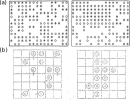
\includegraphics[width=0.7\textwidth]{Figs/Introduction/schelling_diagrams.png}
    \caption[Schelling and Sakoda checkerboard examples]{\textbf{(a)} Examples of the dynamics in Schelling's Segregation Model (from Schelling's original work \cite{Schelling}). \textbf{(b)} Examples of the dynamics in Sakoda’s Checkerboard Conceptual Model (from Sakoda's original work \cite{sakoda1949minidoka}).}
    \label{fig:Schelling_fig}
\end{figure}

Thomas C. Schelling's segregation model \cite{schelling-1969}, introduced in 1969, represents a key innovation in the use of agent-based modeling to explore social phenomena \cite{hegselmann-2017}. Schelling's model illustrates how individual preferences regarding neighbors can inadvertently lead to significant racial segregation in urban areas, even when these preferences are relatively mild. The model utilizes a checkerboard setup where each agent (representing a household) prefers to live in a neighborhood where at least a certain percentage of neighbors are of the same type (see Fig. \ref{fig:Schelling_fig}). Agents move to a new location if their tolerance threshold is not met. This simple rule leads to complex patterns, showing that even a slight preference for similar neighbors can result in highly segregated communities, an insight that has profound implications for understanding social dynamics and urban planning.

\begin{theorem}[Schelling's model]
    An individual time step of the model is defined as follows:
    \begin{enumerate}
        \item Each node $i$ has a tolerance threshold $T_i$.
        \item At each time step, a node $i$ is selected at random.
        \item If the fraction of different kind neighbors of $i$ is greater than $T_i$, then $i$ moves to a neighboring location where the fraction of different kind neighbors is less than $T_i$.
            \begin{itemize}
                \item If there is no available location, then $i$ remains in the same location.
            \end{itemize}
    \end{enumerate}
\end{theorem}

James M. Sakoda's model, initially conceptualized in his 1949 dissertation and fully introduced in Ref. \cite{sakoda1971checkerboard} pre-dates Schelling's work and offers a more nuanced approach to modeling social interactions using a similar checkerboard framework. Unlike Schelling's focus solely on segregation dynamics, Sakoda's model incorporates a broader range of social interactions by allowing agents to exhibit positive, neutral, or negative attitudes towards their neighbors. These attitudes influence the agents' movements across the board, aiming to optimize their local environment according to specific utility functions that aggregate the effects of surrounding agents. Sakoda's model is capable of simulating a variety of social phenomena beyond segregation, such as the formation of stable social clusters and the dynamics of group interactions \cite{hegselmann-2017}. 

Both models employ a checkerboard as the computational space where agents (or tokens) reside and interact according to predefined rules. The ``hand-made'' simulations performed by Sakoda and Schelling using a checkerboard discrete representation has since become a standard framework for studying agent-based models in social systems \cite{hegselmann-2017}. The checkerboard structure allows for the exploration of local interactions and the emergence of global patterns, providing a powerful tool for understanding the dynamics of social systems.

\begin{theorem}[Sakoda's model]
    An individual time step of the model is defined as follows:
    \begin{enumerate}
        \item Each node $i$ has an attitude matrix $A_i$.
        \item At each time step, a node $i$ is selected at random.
        \item $i$ evaluates the total utility for each neighboring location based on the sum of influences from all other agents on the board, weighted by distance.
        \item $i$ moves to the location with the highest utility.
        \begin{itemize}
            \item If there is no available location, then $i$ remains in the same location.
        \end{itemize}
    \end{enumerate}
\end{theorem}

The results of the Schelling's model demonstrated how even mild personal preferences can unexpectedly lead to significant societal segregation. Its insights have been applied across economics, sociology, urban planning, and complexity science, profoundly influencing both academic research and practical policy discussions. Schelling's model became a foundational example in agent-based modeling, helping to educate countless researchers and practitioners about the impact of individual actions on broader social patterns. This contribution was one of the key reasons Schelling was awarded the Nobel Prize in Economics in 2005, underscoring the model's enduring influence and importance. Nevertheless, when we check the update rules, we observe that the Schelling's model is a particular case of the previous Sakoda's model, where agents have a negative attitude towards different-kind agents and a fixed tolerance threshold. To honor the original contributions of both authors, we refer to this model as the Sakoda-Schelling model.

In particular, the Sakoda-Schelling model has been studied from a Statistical Physics point of view due to its close relation to different forms of Kinetic Ising-like models \cite{stauffer-2007,stauffer-2013}, and also addressing general questions of clustering and domain growth phenomena, as well as for the existence of phase transitions from segregated to non-segregated phases. For example, the relation with phase separation in binary mixtures has been considered \cite{Dall_Asta_2008,Vinkovic}, as well as the connection with the phase diagram of spin-1 Hamiltonians \cite{BEG,BlumeCapel,Gauvin_2009,Gauvin_2010}. In this context a useful classification of models is to distinguish between two possible types of dynamics \cite{Dall_Asta_2008}: ``constrained'', where agents just move to satisfying vacancies (if possible), and ``unconstrained'',  where agents' motion does not prevent them to remain unsatisfied. In addition, the motion can be short-range (only to neighboring sites, as in the original model) or long-range. Constrained motion has been named ``solid-like'' because it generally leads to frozen small clusters, while unconstrained motion has been considered ``liquid-like'' because it allows for large growing clusters \cite{Vinkovic}. Including the motion of satisfied agents leads to a noisy effect playing the role of temperature in a statistical physics approach. 

\section{\label{sec: Bursty Human Dynamics} Bursty Human Dynamics}

Bursty human behavior refers to the irregular and heterogeneously timed activity patterns observed in various human interactions, including communication, mobility, and social dynamics. This manuscript provides an overview of bursty behavior, reviews empirical evidence supporting its existence, and discusses its implications for modeling human behavior within network science.


Human activities often exhibit complex temporal patterns that are characterized by bursts—short periods of high activity followed by long periods of inactivity. This non-Poissonian behavior, referred to as burstiness, is a common trait in various human-driven processes and has been widely observed in the dynamics of communication, web browsing, and social interactions \cite{Barabasi2005Bursts, Vazquez2006Bursts}.

The concept of bursty behavior in human dynamics was first significantly highlighted by \cite{Barabasi2005Bursts}, where it was shown that the timing of tasks such as email correspondence does not follow a regular pattern but is instead characterized by bursts. Further studies expanded these findings across different types of data, such as mobile phone calls and text messages, demonstrating that such patterns are ubiquitous in human interactions \cite{Karsai2012Spreading, Miritello2013Capacity}.

\cite{Eckmann2004Entropy} analyzed email communication to demonstrate that the burstiness can be attributed to the structured nature of human dialogue, where the response times play a crucial role in the entropy and coherence of email traffic.

Understanding bursty dynamics is crucial for modeling various phenomena in network science, including the spread of information, disease modeling, and social influence. Traditional models based on Poisson processes often fall short in capturing the real dynamics due to their assumption of uniform activity rates. To address this, models incorporating non-Poissonian statistics have been developed \cite{Vazquez2006Bursts}.

\begin{figure}
    \centering
    \captionsetup{font=sf}
    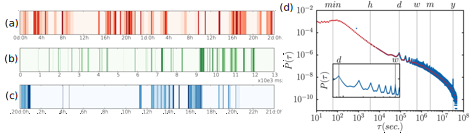
\includegraphics[width=\textwidth]{Figs/Introduction/bursty.png}
    \caption[Bursty human dynamics: examples and distribution]{}
    \label{fig:bursty_human_dynamics}
\end{figure}

Activity-driven modeling approaches, for instance, incorporate the temporal aspects of human activity by assigning activity potentials to each node in a network, which dictate the likelihood of interactions based on empirical observations of human activity \cite{Perra2012ActivityDriven}. This approach not only captures the burstiness but also allows for the modeling of diffusion processes more accurately.

\cite{Jo2012Circadian} and \cite{Starnini2013FaceToFace} further demonstrated that burstiness could be modulated by circadian rhythms and face-to-face interactions, suggesting the necessity to integrate these factors into predictive models.

The presence of bursty behavior has significant implications for the dynamics of processes conducted over networks. For instance, the spread of epidemics can be heavily influenced by the timing and frequency of human interactions \cite{Rocha2013Bursts}. Similarly, information diffusion, online social contagions, and even the spread of mobile phone viruses are impacted by these temporal patterns \cite{Wang2009Viruses, Lazer2009CompSocSci}.

Moreover, understanding burstiness helps in designing better communication strategies and improving technological infrastructures by aligning them more closely with natural human activity patterns.

Bursty human behavior is a fundamental aspect of human dynamics that affects various processes within network science. Accurate modeling of these behaviors is essential for predicting and managing the complex systems that characterize modern interconnected societies.

Moreover, understanding burstiness helps in designing better communication strategies and improving technological infrastructures by aligning them more closely with natural human activity patterns.

Bursty human behavior is a fundamental aspect of human dynamics that affects various processes within network science. Accurate modeling of these behaviors is essential for predicting and managing the complex systems that characterize modern interconnected societies.

---------------

- All models previously described are based in an important assumption regarding to its dynamics: the interactions between individuals occur at a constant rate.

- This constant rate assumption is assuming that the stochastic interactions follow a Poisson process. 

- However, from the analysis of many datasets of human interactions, it has been observed that the interactions between individuals are not constant, but bursty.

- The bursty behaviour is characterized by power law interevent time distributions, and it is present in many human activities, such as e-mail communication, face-to-face interactions, and phone calls.

- The modeling of bursty human dynamics is important because it allows us to understand how the bursty behaviour of human interactions affects the dynamics of social systems.

- Previous literature has several approaches to model bursty human dynamics: temporal networks, activity-driven models, aging \dots

\section{\label{sec:Aging mechanism} Aging mechanism}

- The aging mechanism is a mechanism that has been proposed to model the bursty behaviour of human interactions.

- Aging mechanism is based on the idea that the probability of an individual to interact with another individual decreases with the time since the last interaction.

- Attachment to previous beliefs or habits is a common feature in human behavior. Granovetter (1973) discussed 

- Instead of the constant rate assumption, the aging mechanism assumes that the interactions between individuals occur at a rate that decreases with the time since the last interaction.

- The focus on this approach is to include the bursty dynamics in the individuals attempts to interact with others, rather than in the interactions themselves (as in the activity-driven models or temporal networks).

It is known that human interactions do not occur at a constant rate. They rather show  a bursty character with a non-Poissonian inter-event time distribution that reflects a memory from past interactions. \cite{barabasi-2005,moro,oriol,rybski-2012,zignani-2016,kumar-2020}
However, most social simulations, including simulations of variants of the Sakoda-Schelling model, implicitly assume a constant rate of interactions or state updating. "Aging" is one form of memory effect on which the rate of interactions depends on the persistence time of an agent in a state, modifying the transition to a different state \cite{fernandez-gracia-2011,perez-2016,boguna-2014}. This concept of aging, or "social inertia" \cite{Stark2008}, constrains the transitions in a way that the longer an agent remains in a given state, the smaller the probability to change it. Aging has been already shown to modify social dynamics very significantly. For example, in opinion dynamics, aging is able to produce coarsening towards a consensus state in the voter model \cite{fernandez-gracia-2011,peralta-2020} or to induce a continuous phase transition in the noisy voter model \cite{artime-2018}.

Aging is an important non-Markovian effect that we address in this chapter for binary-state models. Aging accounts for the influence that the persistence time of an agent in a given state modifies the transition rate to a different state \cite{stark-2008,fernandez-gracia-2011,perez-2016,boguna-2014,chen-2020}, so that, the longer an agent remains in a given state, the smaller is the probability to change it. 

Aging effects have been already shown to modify binary-state dynamics very significantly. For example, aging is able to produce coarsening towards a consensus state in the Voter model \cite{fernandez-gracia-2011,peralta-2020C}, to induce continuous phase transitions in the noisy Voter model \cite{artime-2018,peralta-2020A}.

\section{\label{sec:Aging in Simple Contagion Models} Aging in Simple Contagion Models}

- Aging in the Voter model has been studied by many authors, and it has been shown that the aging mechanism affects the dynamics of the model.

- The aging mechanism has been shown to affect the dynamics of the Voter model, and to change the phase transition of the model.

- Aging in the noisy voter model is able to change the phase transition of the model, and to make the phase transition continuous.

- Aging in the SI model is able to change the cascade size distribution of the model, and to make the cascade size distribution follow a power law (see the work of Karsai et al. 2011).